\documentclass[aspectratio=169]{beamer}
\usetheme{Madrid}

\title{Request Batching with Predictive Dyna-Q}
\author{Ashrith}
\date{\today}

\begin{document}

% Slide 1: Architecture + Methodology
\begin{frame}{Architecture and Methodology}
\small
\textbf{System Architecture}
\begin{itemize}
    \item \textbf{Input State (6D):} batch size, wait time, queue length, time since last skip, arrival rate, system load
    \item \textbf{Predictive Layer:} grouped linear predictor estimates near-future demand
    \item \textbf{Decision Layer:} Predictive Dyna-Q policy chooses \texttt{WAIT} (0) or \texttt{SKIP} (1)
    \item \textbf{Environment Feedback:} reward and next state update Q-table + planning model
\end{itemize}

\vspace{0.2cm}
\textbf{Methodology}
\begin{itemize}
    \item Train/evaluate on \texttt{poisson}, \texttt{bursty}, and \texttt{time\_varying} traffic
    \item Evaluate across 5 seeds with aggregated metrics
    \item Core metrics: mean reward, avg wait, P95 wait, avg batch size, throughput, SLO violation rate
\end{itemize}
\end{frame}

% Slide 2: Scores + Metrics
\begin{frame}{Scores and Final Metrics (Aggregated)}
\scriptsize
\begin{table}
\centering
\begin{tabular}{lcccc}
\hline
\textbf{Model} & \textbf{Mean Reward} & \textbf{Avg Wait (s)} & \textbf{P95 Wait (s)} & \textbf{SLO Viol. (\%)} \\
\hline
REINFORCE & -2.07 & 0.244 & 0.453 & 0.0 \\
A2C & -25.81 & 1.099 & 2.018 & 54.9 \\
PPO & -26.22 & 1.109 & 2.025 & 55.5 \\
Predictive Dyna-Q & -29.96 & 0.587 & 1.518 & 24.5 \\
Fixed Wait (1.0s) & -14.70 & 0.646 & 1.100 & 22.1 \\
Random & -10.82 & 0.330 & 0.869 & 3.2 \\
\hline
\end{tabular}
\end{table}

\vspace{0.15cm}
\footnotesize
\textbf{Notes:}
\begin{itemize}
    \item Throughput for all methods remains around 6.6--6.8 req/s.
    \item Main optimization target was latency-quality tradeoff under variable demand.
\end{itemize}
\end{frame}

% Slide 3: Placeholders for user images
\begin{frame}{Agent comparision plot}
\begin{columns}[T]

    \column{0.8\textwidth}
    \centering
    
\includegraphics[width=\linewidth,height=0.8\textheight,keepaspectratio]{comparison.png}\\
    \scriptsize comparative metrics plot
\end{columns}
\end{frame}

\begin{frame}{Training curves}
\begin{columns}[T]
    \column{0.49\textwidth}
    \centering
    \textbf{}\\[0.1cm]
    
\includegraphics[width=\linewidth,height=0.8\textheight,keepaspectratio]{training_curves.png}\\
    \scriptsize 

    \column{0.49\textwidth}
    \centering
    \textbf{}\\[0.1cm]
    \includegraphics[width=\linewidth,height=0.8\textheight,keepaspectratio]{training_curves_2.png}\\
    \scriptsize
\end{columns}
\end{frame}

\begin{frame}{Live simulation plots}
\begin{columns}[T]
    \column{0.49\textwidth}
    \centering
    \textbf{}\\[0.1cm]
    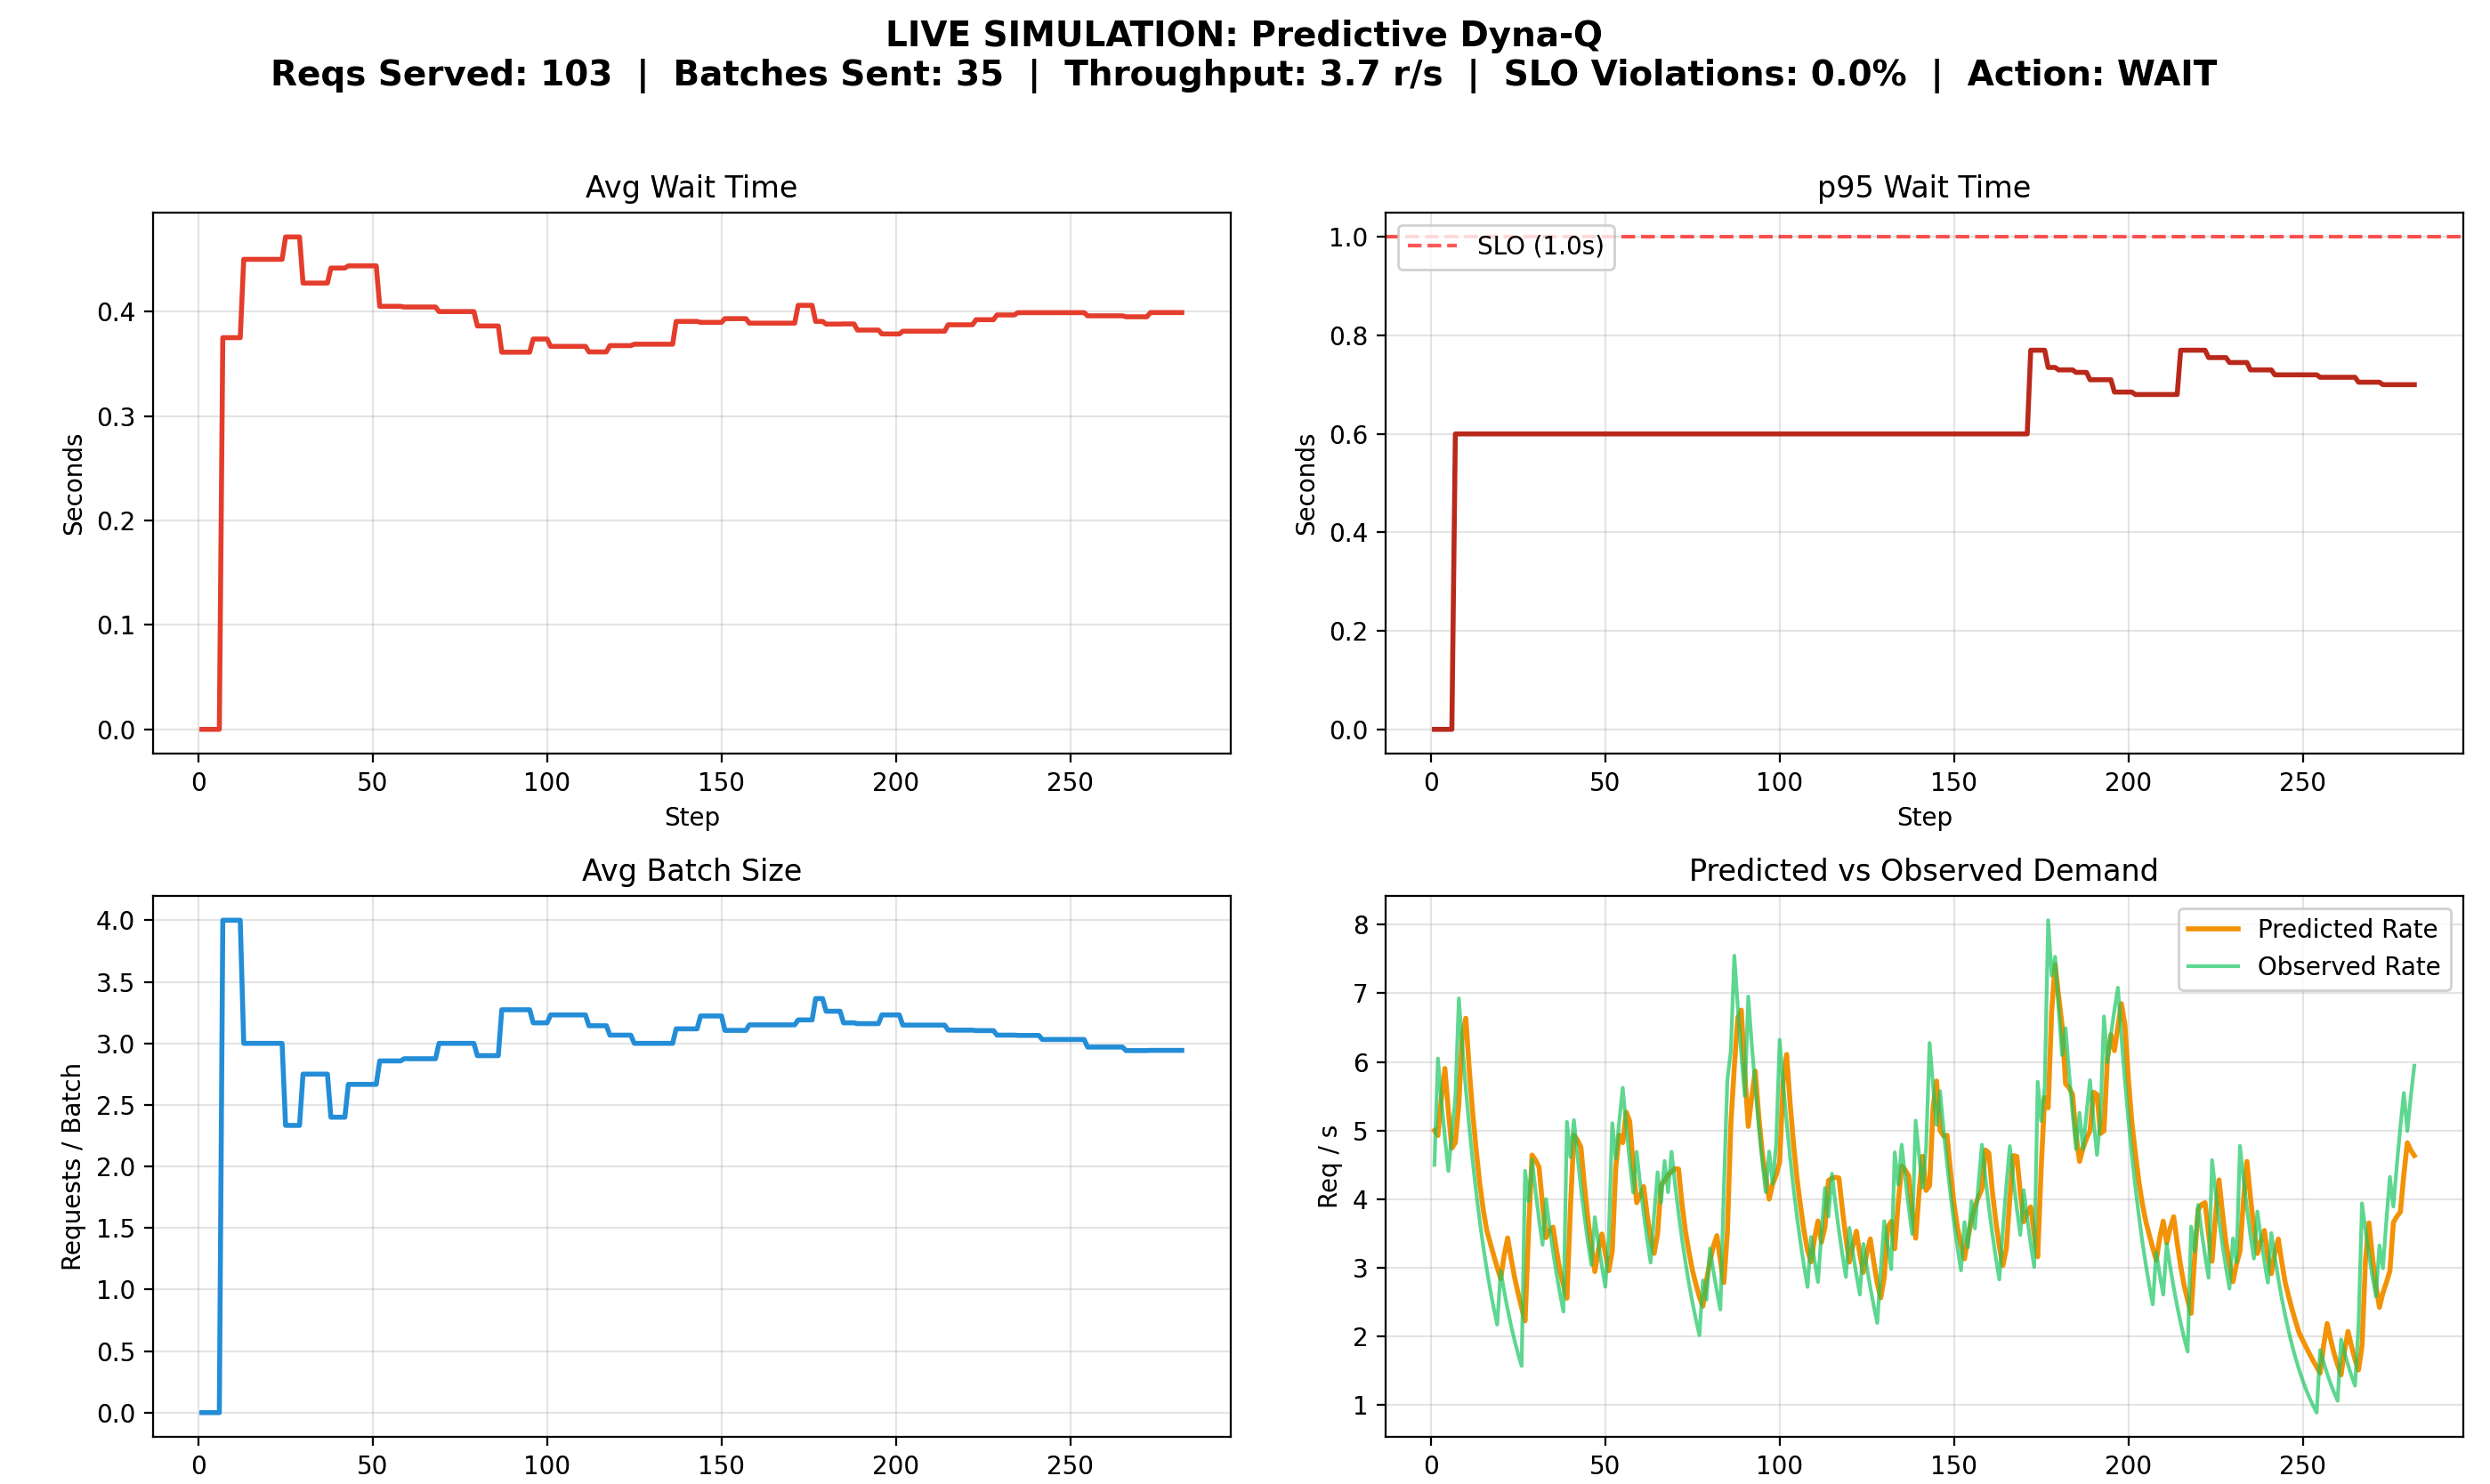
\includegraphics[width=\linewidth,height=0.7\textheight,keepaspectratio]{Screenshot 2026-05-13 at 8.01.20 PM.png}\\
    \scriptsize 103 requests served.

    \column{0.49\textwidth}
    \centering
    \textbf{}\\[0.1cm]
    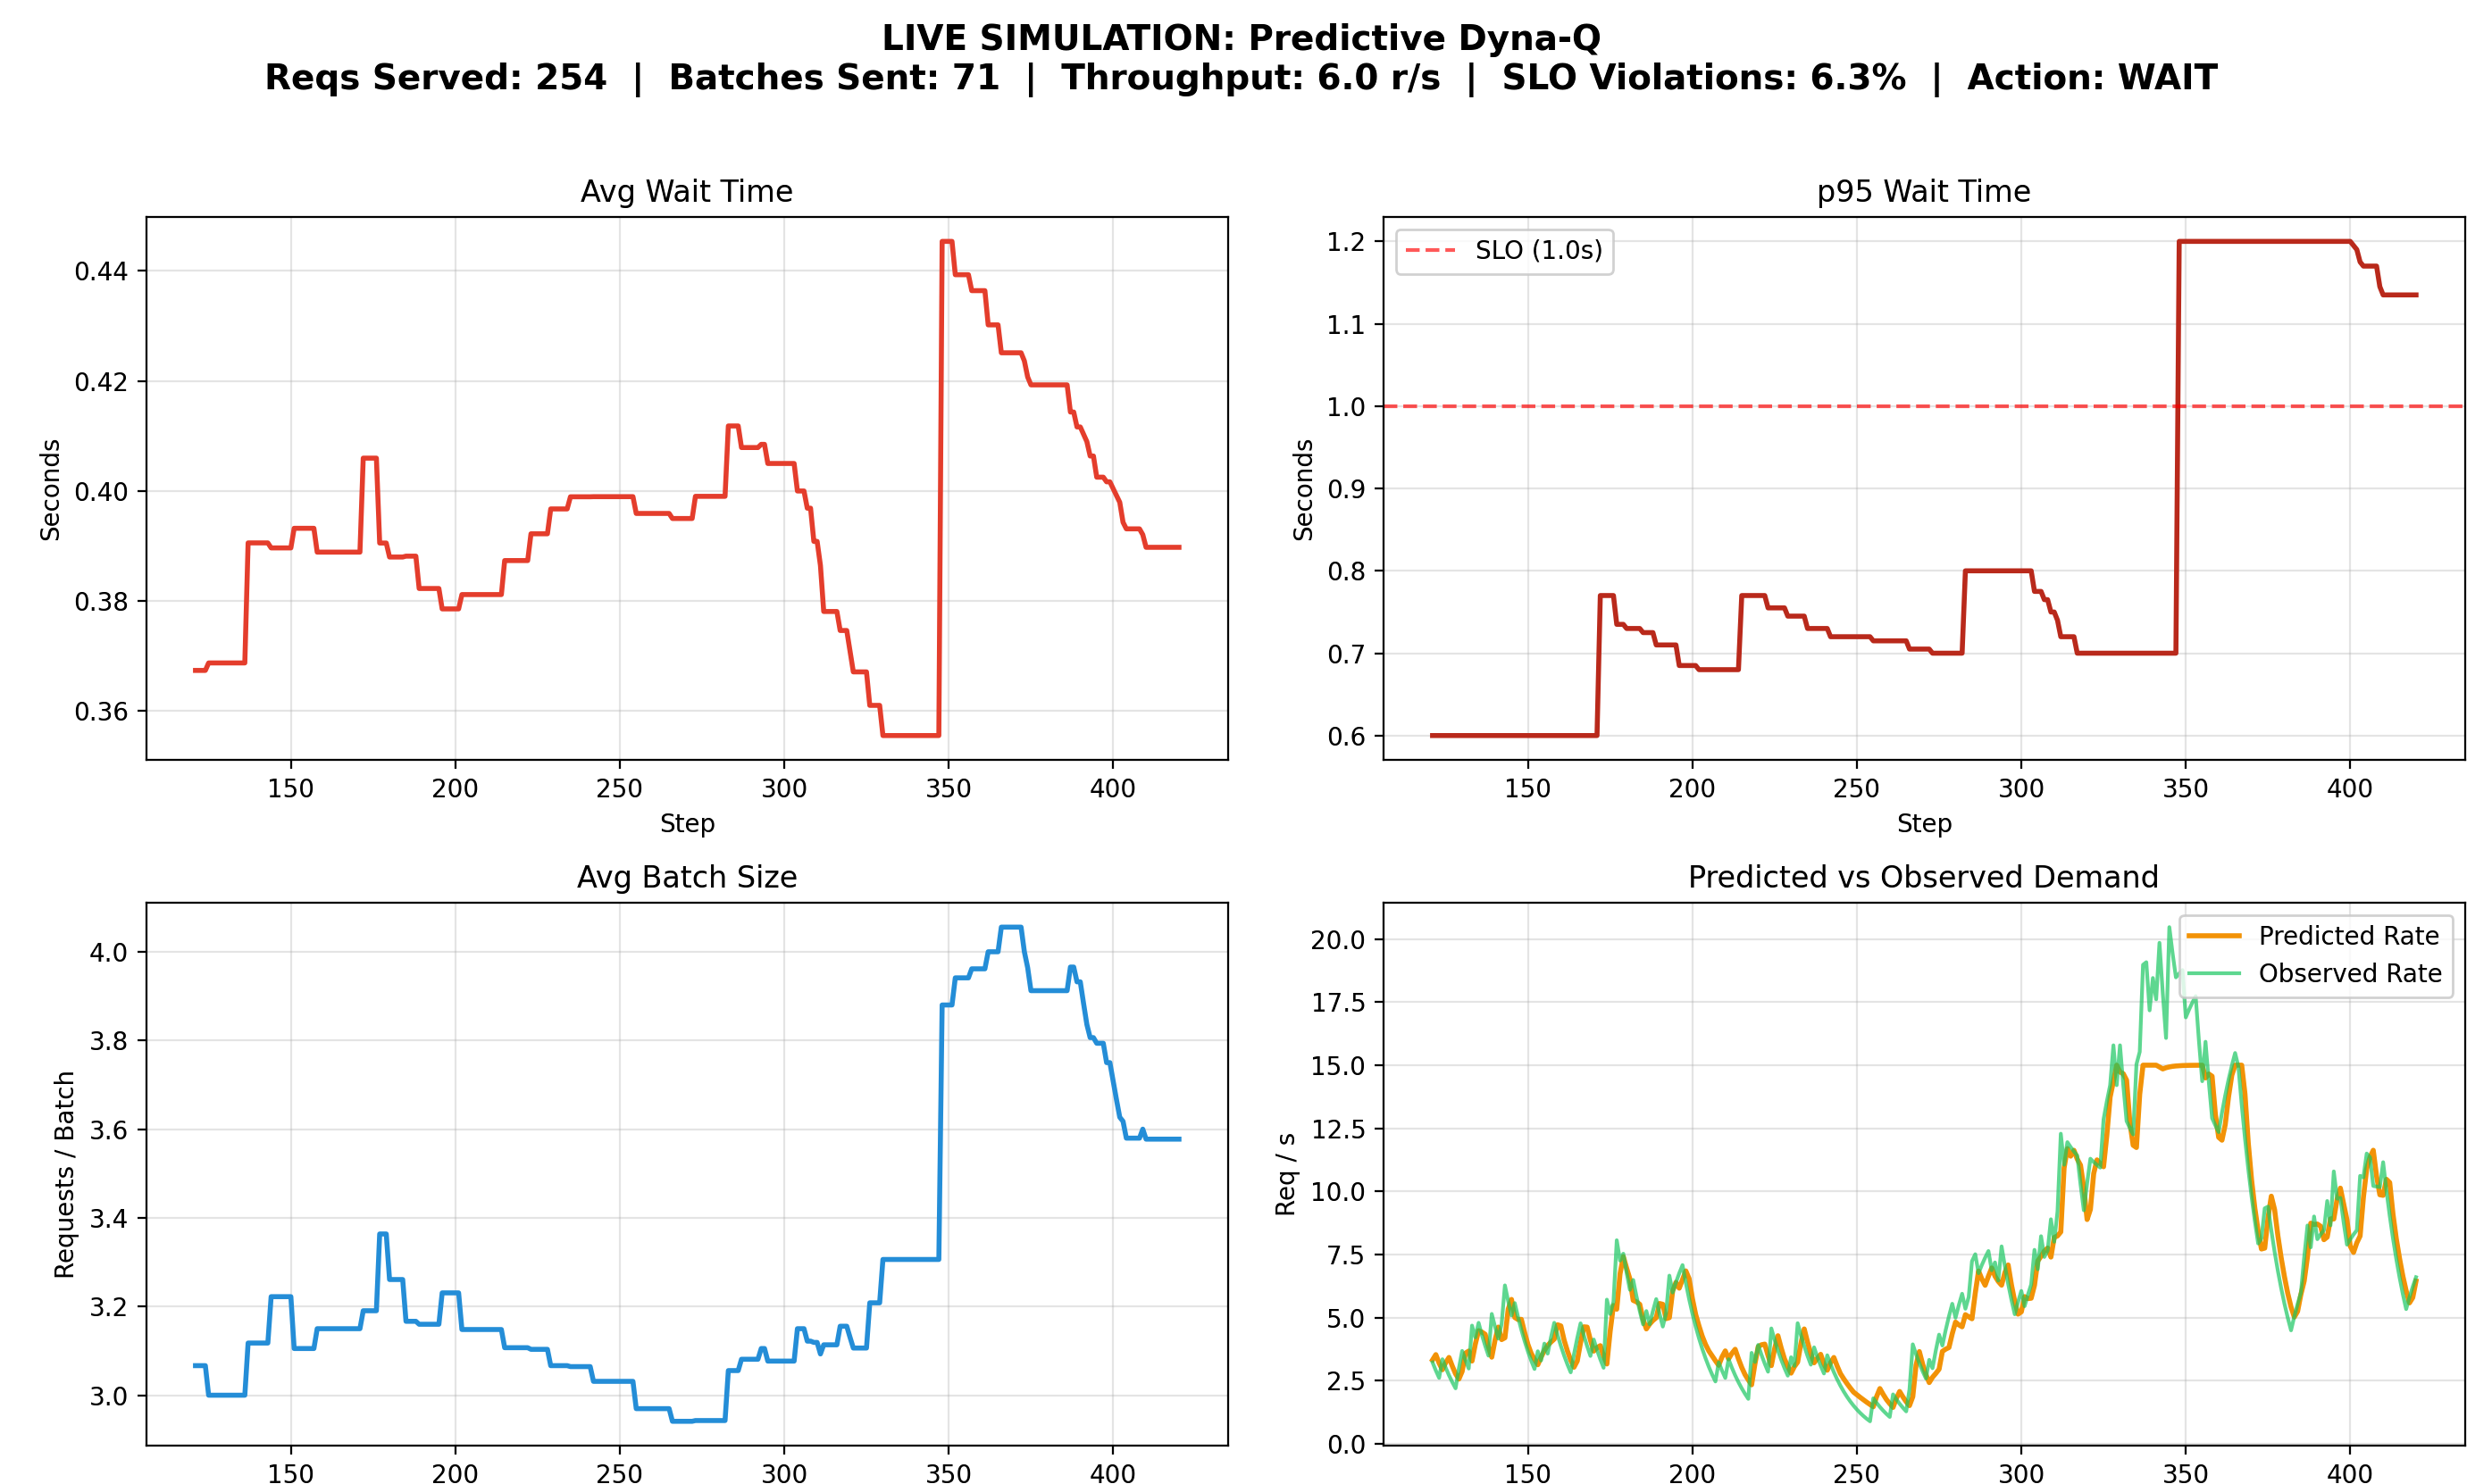
\includegraphics[width=\linewidth,height=0.7\textheight,keepaspectratio]{Screenshot 2026-05-13 at 8.01.48 PM.png}\\
    \scriptsize 254 requests served.
\end{columns}
\end{frame}

\end{document}